\documentclass[11pt]{book}
\usepackage{palatino}
% \usepackage{amsfonts,amsmath,amssymb}
\usepackage{graphicx}
\usepackage{epstopdf}

% Packages for Figures:
%\ifx\pdftexversion\undefined
%    \usepackage[dvips]{graphicx}
%\else
%    \usepackage[pdftex]{graphicx}
%    \usepackage{epstopdf}
%    \epstopdfsetup{suffix=}
%\fi

% Packages for displaying code:
\usepackage{listings}
\usepackage{textcomp}
\usepackage{color}

% Color settings used in the code below:
\definecolor{dkgreen}{rgb}{0,0.6,0}
\definecolor{gray}{rgb}{0.5,0.5,0.5}
\definecolor{mauve}{rgb}{0.58,0,0.82}

% Settings for the formatting of the code on display:
\lstset{frame=tb,
  language=R,
  aboveskip=3mm,
  belowskip=3mm,
  showstringspaces=false,
  columns=flexible,
  basicstyle={\small\ttfamily},
  numbers=none,
  numberstyle=\tiny\color{gray},
  keywordstyle=\color{blue},
  commentstyle=\color{dkgreen},
  stringstyle=\color{mauve},
  breaklines=true,
  breakatwhitespace=true,
  tabsize=3
}

% Package for displaying inline verbatim commands in footnotes.
\usepackage{fancyvrb}


\begin{document}

%%%%%%%%%%%%%%%%%%%%%%%%%%%%%%%%%%%%%%%%
% Problem Set 4
%%%%%%%%%%%%%%%%%%%%%%%%%%%%%%%%%%%%%%%%

\pagestyle{empty}
{\noindent\bf Spring 2021 \hfill Firstname M.~Lastname}
\vskip 16pt
\centerline{\bf University of Central Florida}
\centerline{\bf College of Business}
\vskip 16pt
\centerline{\bf QMB 6911}
\centerline{\bf Capstone Project in Business Analytics}
\vskip 10pt
\centerline{\bf Solutions:  Problem Set \#5}
\vskip 32pt
\noindent

\section{Introduction}

This note summarizes the findings in the script
\texttt{Tractor\_Data\_Vis.R},
which analyzes the prices of fly reels,
the dependent variable in the \texttt{TRACTOR7.csv} dataset.
The output includes several plots of the 
dependent variable against the explanatory variables.

The primary goal is to determine the relative value of John Deere tractors compared to others. 
A secondary consideration is to determine the time of year in which to 
sell a tractor. 

\vfill
\pagebreak
\section{Histogram and Density of Log. Fly Reel Prices}


\subsection{All Tractors Together}

Start with the log of sale prices because that
seemed more promising, given that prices were highly skewed.

\begin{lstlisting}[language=R]
hist(tractor_sales[, 'log_saleprice'],
     main = 'Histogram and Density of Log. Tractor Prices',
     xlab = 'Price',
     col = 'red',
     probability = TRUE)
rug(tractor_sales[, 'log_saleprice'])
lines(density(tractor_sales[, 'log_saleprice']),
      col = 'blue',
      lwd = 3)
\end{lstlisting}


Figure \ref{fig:hist_dens_log_price} is
a histogram of the logarithm of tractor prices, 
along with a rug plot and a kernel density estimate, 
generated by the code block above.
%
\begin{figure}[h!]
  \centering
  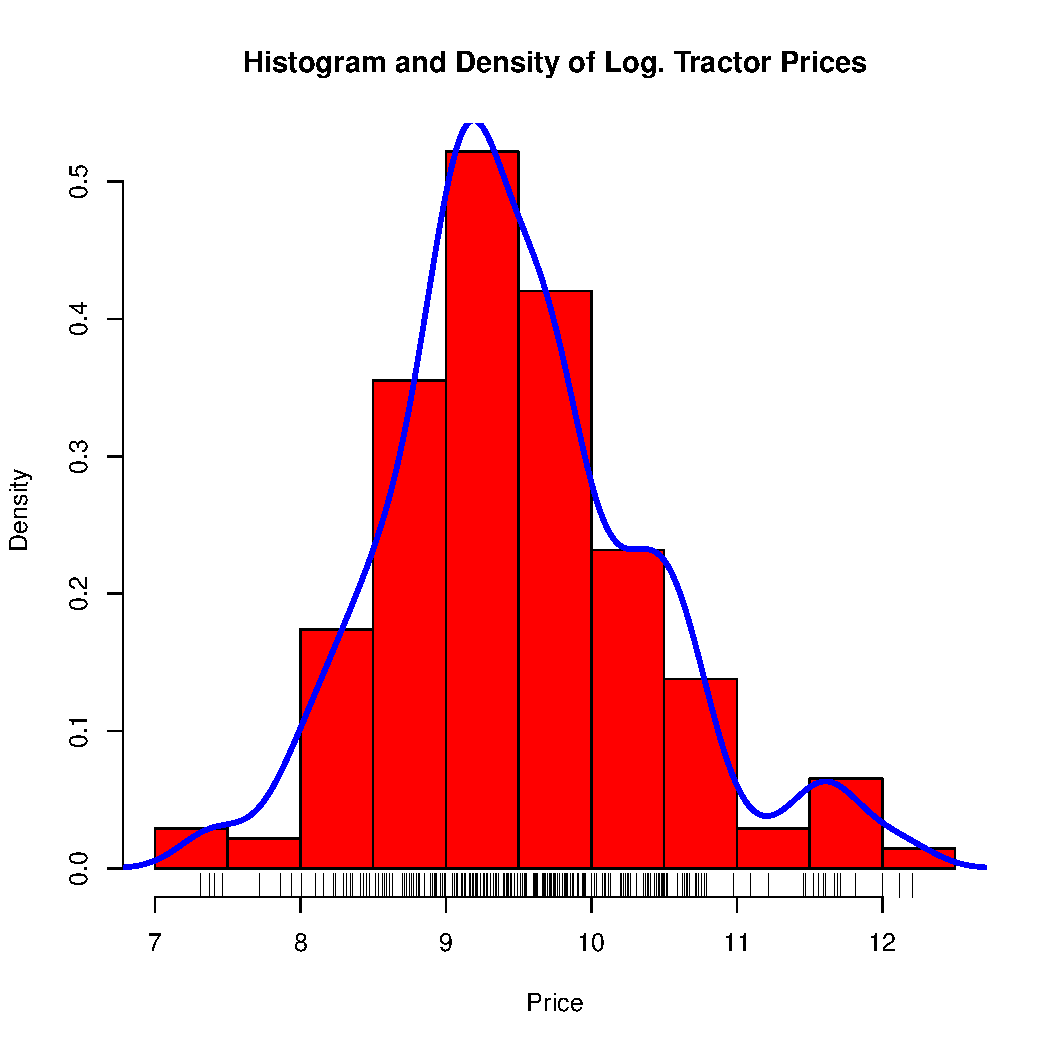
\includegraphics[scale = 0.5, keepaspectratio=true]{../Figures/hist_dens_log_price}
  \caption{Relative Histogram of Tractor Prices} \label{fig:hist_dens_log_price}
\end{figure}
% 
After taking logs, we can see that the distribution is
approximately symmetric, with some bunching in the
upper tail. 

\pagebreak
\subsection{Comparison By Make}

Now we investigate the value of John Deere tractors 
compared to other brands.
Figure \ref{fig:dens_by_brand} shows the 
kernel density estimate of the sale prices of John Deere tractors
in green and that of the other brands in red.
% 
The distribution of sale prices of John Deere tractors has several modes and is skewed to the right, 
with the highest mode lower than that for other brands. 


\begin{lstlisting}[language=R]
library(sm)
sm.density.compare(tractor_sales[, 'log_saleprice'],
                   tractor_sales[, 'johndeere'],
                   xlab = "Log. of Sale Price",
                   lwd = 3,
                   col = c('red','green'))
title(main = "Log. of Sale Price by Brand")
legend('topright', c('Other', 'John Deere'),
       fill = c('red','green'),
       cex = 0.75)
\end{lstlisting}


\begin{figure}[h!]
  \centering
  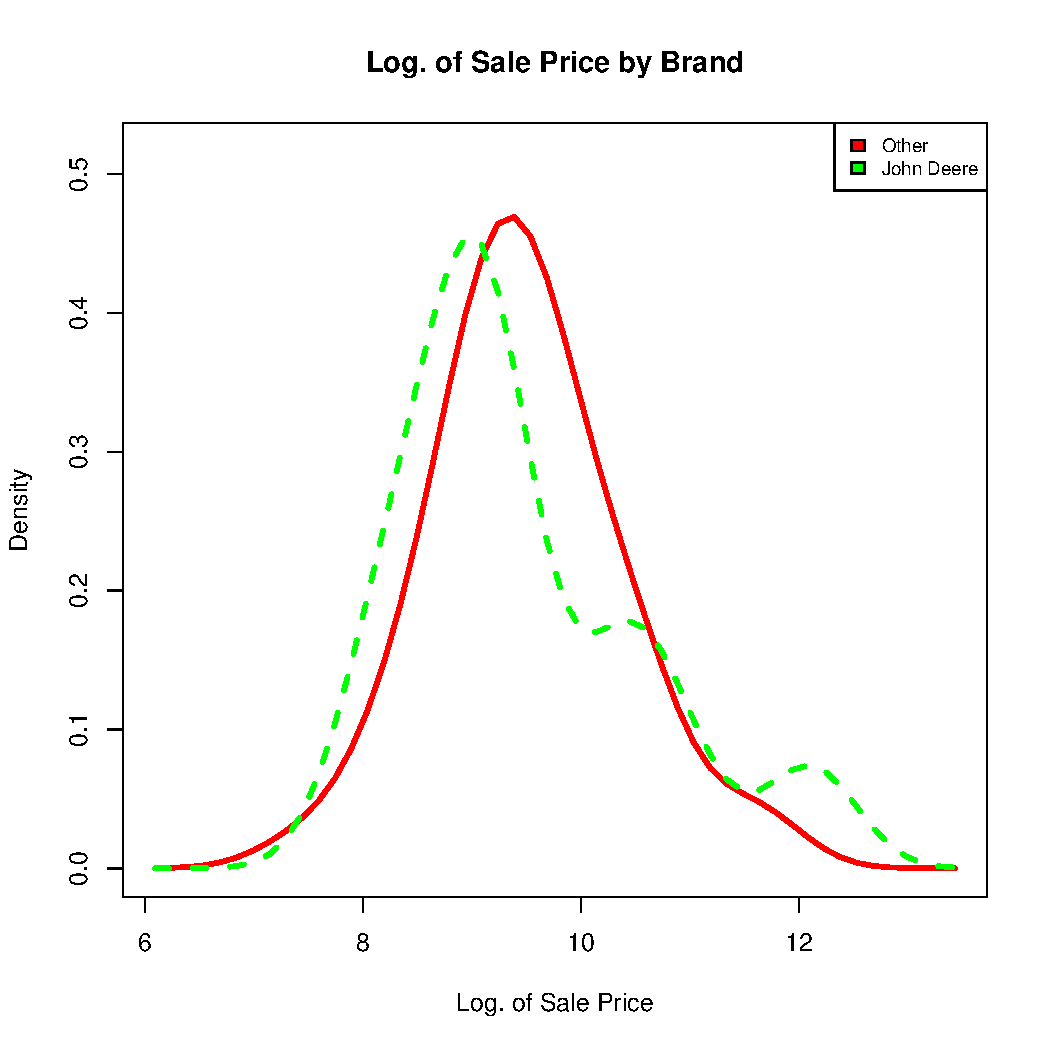
\includegraphics[scale = 0.5, keepaspectratio=true]{../Figures/dens_by_brand}
  \caption{Densities of Log. Tractor Prices by Brand} \label{fig:dens_by_brand}
\end{figure}


\pagebreak
\subsection{Comparison By Season of Sale}

Figure \ref{fig:dens_by_season} shows 
the densities of the logarithm of sales price,
separated by the season of the year in which they were sold.
The figure was generated by the following code.
% 

\begin{lstlisting}[language=R]
plot(density(tractor_sales[tractor_sales[, 'fall'] == 1, 'log_saleprice']),
     col = 'orange',
     lwd = 3,
     xlim = c(min(tractor_sales[, 'log_saleprice']),
              max(tractor_sales[, 'log_saleprice'])),
     main = 'Log. of Sale Price by Season of Sale')
# Plot the rest.
lines(density(tractor_sales[tractor_sales[, 'spring'] == 1, 'log_saleprice']),
     col = 'green',
     lwd = 3)
lines(density(tractor_sales[tractor_sales[, 'summer'] == 1, 'log_saleprice']),
      col = 'yellow',
      lwd = 3)
lines(density(tractor_sales[tractor_sales[, 'winter'] == 1, 'log_saleprice']),
      col = 'blue',
      lwd = 3)
legend('topright',
       c('Spring', 'Summer', 'Fall', 'Winter'),
       fill = c('green', 'yellow', 'orange', 'blue'),
       cex = 0.65)
\end{lstlisting}

\pagebreak
We see that the distribution of sales is similar
during summer and fall (yellow and orange, respectively)
with some bunching in the upper tail.
We also see more variance in the sale price in winter,
shown in blue.
In the spring, shown in green, the mode of the distribution
is higher.

\begin{figure}[h!]
  \centering
  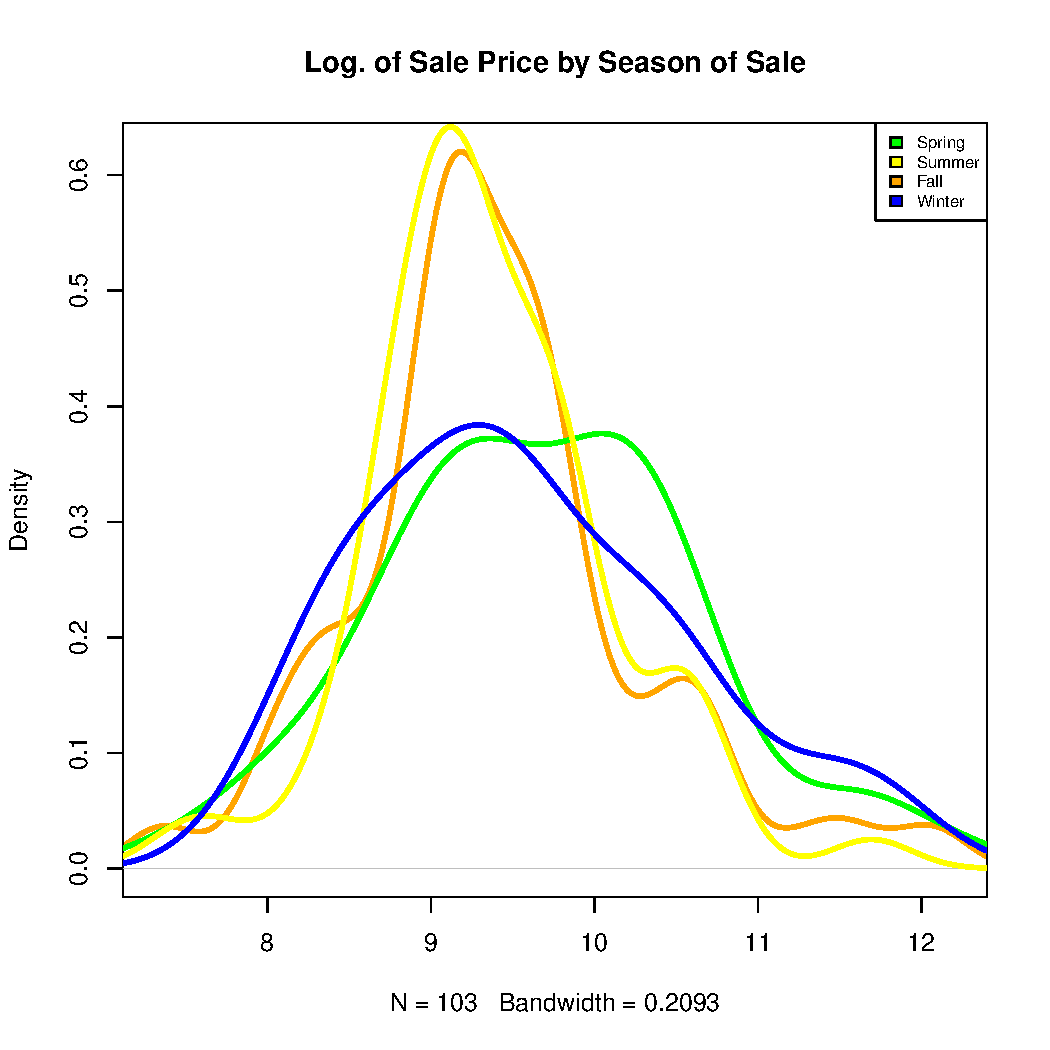
\includegraphics[scale = 0.5, keepaspectratio=true]{../Figures/dens_by_season}
  \caption{Relative Histogram of Tractor Prices} \label{fig:dens_by_season}
\end{figure}


\pagebreak
\section{Sales Volume By Brand and Season of Sale}

Figure \ref{fig:brand_and_season_sales}
shows a spinogram of the number of sales
by brand and the time of year the tractor is sold. 
It is generated by the following code.

\begin{lstlisting}[language=R]
# Create a table and plot it in a spinogram.
counts <- table(tractor_sales[, 'season'],
                tractor_sales[, 'JD'])

# Plot the spinogram.
spine(counts,
      main = "Spinogram of Sales by Brand and Season")
\end{lstlisting}


% \pagebreak
It appears that sales of John Deere tractors are fairly evenly
distributed throughout the year, 
with more sales of John Deere tractors in the winter months
and a fewer sales in the summer. 


\begin{figure}[h!]
  \centering
  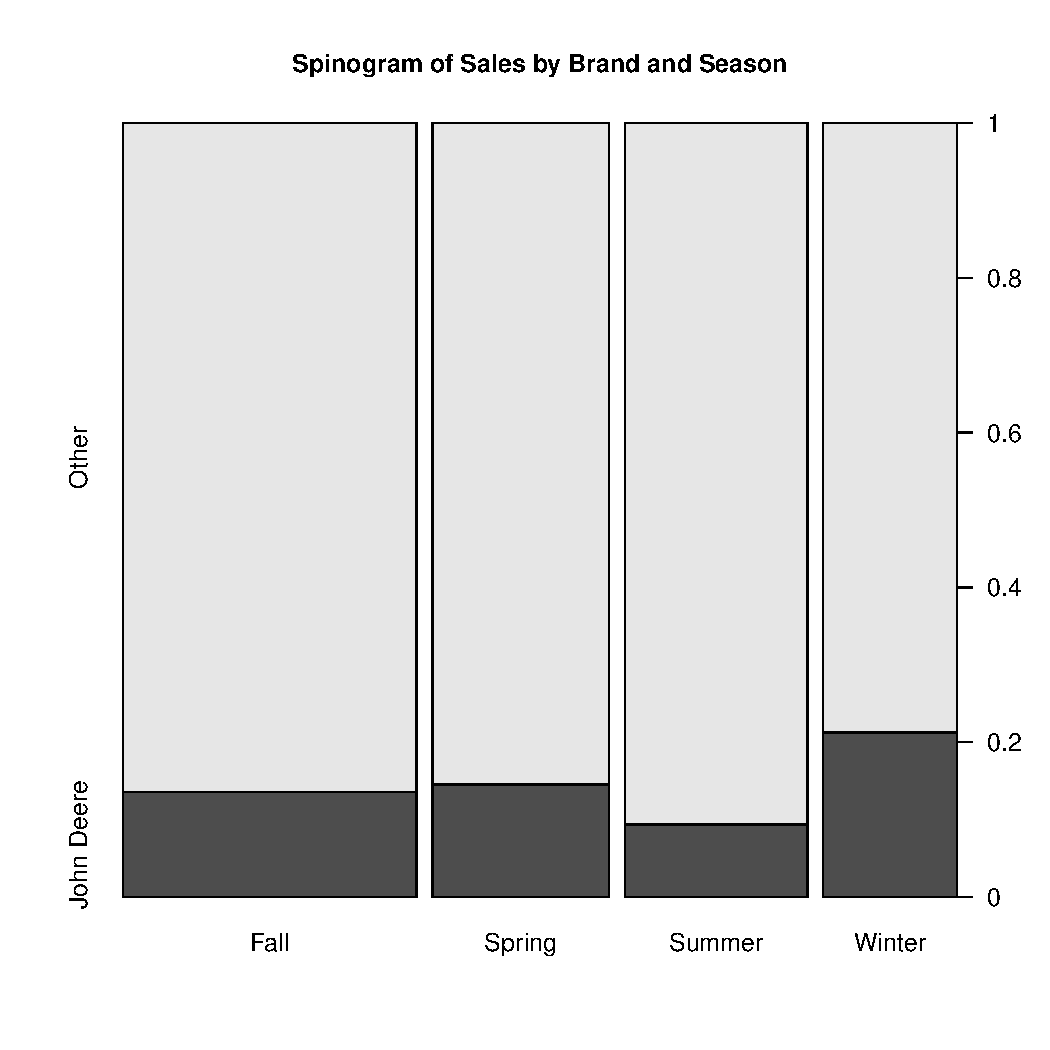
\includegraphics[scale = 0.5, keepaspectratio=true]{../Figures/brand_and_season_sales}
  \caption{Sales Volume of Tractor Prices by Brand and Season of Sale} \label{fig:brand_and_season_sales}
\end{figure}



%%%%%%%%%%%%%%%%%%%%%%%%%%%%%%%%%%%%%%%%
\end{document}
%%%%%%%%%%%%%%%%%%%%%%%%%%%%%%%%%%%%%%%%
